	\documentclass[10pt,oneside]{CBFT_book}
	% Algunos paquetes
	\usepackage{amssymb}
	\usepackage{amsmath}
	\usepackage{graphicx}
% 	\usepackage{libertine}
% 	\usepackage[bold-style=TeX]{unicode-math}
	\usepackage{lipsum}

	\usepackage{natbib}
	\setcitestyle{square}

	\usepackage{polyglossia}
	\setdefaultlanguage{spanish}
	



	\usepackage{CBFT.estilo} % Cargo la hoja de estilo

	% Tipografías
	% \setromanfont[Mapping=tex-text]{Linux Libertine O}
	% \setsansfont[Mapping=tex-text]{DejaVu Sans}
	% \setmonofont[Mapping=tex-text]{DejaVu Sans Mono}

	%===================================================================
	%	DOCUMENTO PROPIAMENTE DICHO
	%===================================================================

\begin{document}

% =================================================================================================
\chapter{Gas de Bose}
% =================================================================================================

Para Bose debe cumplirse $ \mu < \text{ todo } e $ 
y como $ e \geq 0$ eso dice que 
\[
	\mu < 0
\]

Pero si en un sistema tiene $ e_0 $ como mínimo y $ e_0 > 0 $ entonces, ¿puede ser $ \mu > 0 $?
Aparentemente sí (al menos recordando que la restricción sale de la serie).
\notamargen{Ya lo entendí esto: pero no para partícula libre.}

Además $ \braket{n_e} \geq 0 $, el número de partículas debe ser positivo.
\[
	\beta p V = \log (\Xi) = \sum_e - \log ( 1 - \euler^{-\beta(e-\mu)})
\]
\[
	\beta p = \sum_{e \neq 0} \frac{- \log ( 1 - \euler^{-\beta(e-\mu)}) }{V} - \frac{\log (1-z)}{V}
\]

El último término será negligible para todo $z$, incluso con $z\to 1$ pues en ese caso $V \to \infty$ mucho
más rápido
\[
	\braket{n_0} = \frac{1}{z^{-1}-1} = \frac{z}{1-z}
\]
y $ \braket{n_0} / V $ es finito incluso con $z\to 1$, entonces
\[
	\braket{n_0} - z \braket{n_0} - z = 0 \qquad z = \frac{\braket{n_0}}{1+\braket{n_0}}
\]
\[
	1-z = \frac{1}{1+\braket{n_0}}
\]
\[
	- \frac{\log (1-z)}{V} = \frac{\log (1+\braket{n_0})}{V}
\]
 
y dado que $ \log (\braket{n_0}) \ll \braket{n_0} $ despreciamos $ \log (1-z) / V $.

Como $ 0 > \mu $ entonces $ \euler^{\beta \mu} \equiv z < 1 $

En Bose la fugacidad está acotada
\[
	\frac{N}{V} = \frac{1}{\lambda^3} g_{3/2}(z) + \frac{1}{V}\Frac{z}{1-z}
\]
\[
	\frac{\lambda^3}{v} =  g_{3/2}(z) + \frac{\lambda^3}{V} n_0
\]
\[
	\underbrace{\frac{N}{V}}_{\text{ densidad total }} =
	\underbrace{\frac{1}{\lambda^3} g_{3/2}(z)}_{\text{ densidad en los excitados }} +
	\underbrace{\frac{1}{V}\Frac{z}{1-z}}_{\text{ densidad en el fundamental }}
\]

Por otro lado como $ 0 < z < 1 $ entonces $ g_{3/2}(z) $ está acotada 
\[
	g_{3/2}(1) = \sum_{j=1}^\infty \frac{1}{j^{3/2}} = 2.612
\]

Con $z\approx 1$ da
\[
	\frac{\lambda^3}{v} = g_{3/2}(1) + \lambda^3 \frac{n_0}{V} 
\]
cuando se aumenta $N$ necesariamente las partículas se apilan en el fundamental; es una
fracción macroscópica pués $ V \to \infty $ y entonces $ n_0 \to \infty $.

Se da con 
\[
	\frac{\lambda^3}{v} = \frac{\lambda^3}{V} N = \frac{h^3}{(2\pi m kT)^{3/2}} \frac{N}{V} > 2.612
\]
\notamargen{Destaco en esta expresión $T$ baja dividiendo y $n$ alta multiplicando.}

El condensado de Bose surge cuando se saturan los excitados; ello pasa con $T$ baja, $N/V$
alta y $ \mu \to 0$

GRAFIQUETE

El condensado de Bose podemos pensarlo como la coexistencia de dos fluidos ($e=0$ y $e\neq 0$).
Podemos definir un $ T_c, v_c $ desde 
\[
	\frac{\lambda^3}{v} = g_{3/2}(1) = 2.612 = \frac{h^3}{(2 \pi m k T)^{3/2}} \frac{1}{v}
\]
que lleva a que para un dado $v$ tenemos una cierta $T_c$ y para una cierta $T$ tenemos un 
dado $v_c$ dados ambos por 
\[
	T_c^{3/2} = \frac{h^3}{(2 \pi m k T)^{3/2}} \frac{1}{v} \frac{1}{g_{3/2}(1)} \qquad 
	v_c = \frac{\lambda^3(T)}{g_{3/2}(1)}
\]
De esta forma si $ T<T_c$ y $v<v_c$ se tiene la condensación de Bose
\[
	\lambda^3\frac{N}{V} = g_{3/2}(1) + \lambda^3\frac{N_0}{V}
\]
que es válida a partir de la condensación ($T<T_c$)
\[
	N =  \frac{(2 \pi m k )^{3/2}}{h^3} T^{3/2} g_{3/2}(1)  V + N_0 = N \Frac{T}{T_c}^{3/2} + N_0
\]
\notamargen{$N_e = N\Frac{T}{T_c}^{3/2}$}
\[
	N_o = N \left( 1 - \Frac{T}{T_c}^{3/2} \right),
\]
que es válida por supuesto con $T<T_c$.
A partir de haber alcanzado la condensación $z=1$, añadir partículas ($N++$) o reducir el volumen 
($V--$) hace que $N_e/V \to 0 $ pues $V \to \infty$

DIBUJO con observaciones

Cuando $v/\lambda^3$ es chico se saturan los $N_e$ y entonces $ z \to 1 $.

Cuando $v/\lambda^3$ es grande no hay condensado y entonces $ \lambda^3/v \approx z $ o bien
$ 1/ (v/\lambda^3) \approx z $.

Para la presión tendremos
\[
	\beta p = \frac{1}{\lambda^3} g_{5/2}(z)
\]
con $ z = 1 ( T < T_c ) $
\[
	\frac{p}{kT} = \frac{(2\pi m k T)^{3/2}}{h^3} g_{5/2}(1) = 
	\frac{1}{ v (T_c/T)^{3/2} g_{3/2}(1) } g_{5/2}(1)
\]
\[
	p = 1.34 \frac{(2\pi m )^{3/2}}{h^3} (kT)^{5/2} \qquad \qquad 
	\frac{pV}{NkT} = 0.513 \Frac{T}{T_c}^{3/2}
\]
con $ z = 1 ( T = T_c ) $
\[
	\beta p = \frac{ g_{5/2}(1) }{ g_{3/2}(1) v } = \frac{0.513}{v}
\]
\[
	p = 0.513 \frac{NkT}{V} \qquad \text{ es aprox. $1/2 p$ gas ideal clásico }
\]
con $ z \lesssim 1 ( T > T_c ) $
\[
	\beta p = \frac{1}{v} \frac{ g_{5/2}(z) }{ g_{3/2}(z) }
\]
pero no podemos expandir en el virial porque $ \lambda^3 / v $ no es chico.

Con $ z \approx 0 \: ( T \gg T_C ) $
\[
	\beta p v = \frac{pV}{NkT} = \sum_{l=0}^\infty a_l \Frac{\lambda^3}{v}^{l-1}
\]
usando toda la serie y procediendo en modo análogo a Fermi se obtienen
\notamargen{ Los $a_\ell$ son los coeficientes del virial -que son los mismos
para Fermi-.}
\[
	\begin{cases}
	 a_1 = 1 \\
	 a_2 = -0.17678 \\
	 a_3 = -0.00330
	\end{cases}
\]
\[
	\frac{pV}{NkT} = 1 - 0.17678 \Frac{\lambda^3}{v} - 0.00330 \Frac{\lambda^3}{v}^2
\]

DIBUJO 

El virial vale en $\lambda^3/v \ll 1$ (alta $T$ y baja $N/V$ )

A bajas $T$ se comportan de modo muy diferente, $p_{\text{ Fermi }} > 0 $ y
$p_{\text{ Bose }} \approx 0$

% =================================================================================================
\section{Análisis del gas ideal de Bose}
% =================================================================================================

\begin{itemize}
 \item $ \lambda^3 / v \ll 1 $ y entonces $ z \ll 1 $ $\quad  [T \gg T_c ] $
 \[
	\beta p V = \sum_{l=1}^\infty a_l \Frac{\lambda^3}{v}^{l-1} = \frac{ g_{5/2}(z) }{ g_{3/2}(z) }
 \]
 \[
	\beta p V \approx 1 - \frac{\lambda^3}{v} \frac{1}{2^{5/2}} \qquad \qquad 
	U = \frac{3}{2}pV = \frac{3}{2} NkT \left( 1 - \frac{\lambda^3}{v} \frac{1}{2^{5/2}} \right)
 \]
 \item $ \lambda^3 / v \approx 1 $ y entonces $ z < 1 $ $\quad  [T > T_c ] $
 \[
	\beta p V = \frac{ g_{5/2}(z) }{ g_{3/2}(z) }
 \]
 \item  $ \lambda^3 / v = 2.612 $ y entonces $ z = 1 $ $\quad  [T = T_c ] $
 \[
	\beta p V = \frac{ g_{5/2}(z) }{ g_{3/2}(z) } \approx \frac{1.34}{2.612} \approx 0.513
 \]
 \item $ \lambda^3 / v \gg 1 $ y entonces $ z = 1 $ $\quad  [T < T_c ] $ y hay que considerar el 
 fundamental
 \[
	\beta p = \frac{1}{\lambda^3} g_{5/2}(1) \qquad \qquad \lambda^3\Frac{N-N_0}{V} = g_{3/2}(1)
 \]
 \notamargen{Con $z=1$ y $T<T_c$ expresamos todo en términos de $(T/T_c)$.}
 que lleva a 
 \[
	\left( 1 - \frac{N_0}{N} \right) = \Frac{T}{T_c}^{3/2}
 \]
 puesto que $T_c$ es tal que 
 \[
	\frac{h^3}{(2\pi m kT_c)^{3/2}} \frac{N}{V} = g_{3/2}(1) = \frac{\lambda^3}{v}\Frac{T}{T_c}^{3/2}
 \]
 \[
	\beta p V = \frac{ g_{5/2}(z) }{ g_{3/2}(z) } \Frac{T}{T_c}^{3/2} = 0.513 \Frac{T}{T_c}^{3/2}
 \]
 \[
	\frac{\lambda^3}{v} \Frac{T}{T_c}^{3/2} = g_{3/2}(1) \quad \Rightarrow \quad \frac{1}{\lambda^3} =
	\frac{1}{v}\Frac{T}{T_c}^{3/2} \frac{1}{g_{3/2}(1)}
 \]
\end{itemize}

Desde la expresión de la energía $ U = 3/2 p V $ y $C_V = \dpar{}{T}(3/2 p V)$
y entonces
\begin{itemize}
 \item $ T < T_c $ 
 \[
	C_V = \dpar{}{T}\left( \frac{3}{2} N k \Frac{T}{T_c}^{3/2} 0.513  \right) = 
	\frac{15}{4} N k \Frac{T}{T_c}^{3/2} 0.513 \qquad C_V \propto T^{3/2}
 \]
 \item $ T = T_c $ 
 \[
	C_V = N k \; 0.513 \frac{15}{4} = N k 1.92375
 \]
 \item $ T > T_c $ 
 \[
	C_V = \left( \frac{15}{4}\frac{ g_{5/2}(z) }{ g_{3/2}(z) } - 
	\frac{9}{4} \underbrace{\frac{ g_{3/2}(z) }{ g_{1/2}(z) }}_{\to \infty \text{ en } z=1} \right)
 \]
 $C_V$ es continuo.
 \item $ T \gg T_c $ 
 \[
	C_V = N k \frac{3}{2} \dpar{}{T} \left( T \sum_{l=1}^\infty a_l \Frac{\lambda^3}{v}^{l-1} \right)
 \]
 \[
	C_V = N k \frac{3}{2} \left( 1 + 0.0884 \Frac{\lambda^3}{v} + ... \right)
 \]
\end{itemize}

DIBUJO

\subsection{Condensado de Bose como transición de fase}

\[
	\frac{N_0}{N} = 1 - \Frac{T}{T_c}^{3/2}
\]
\[
	\frac{N_0}{N} = 1 - \frac{v}{v_c}
\]
que se obtiene desde las siguientes
\[
	\frac{\lambda^3(T_c)}{v} = g_{3/2}(1) \qquad \qquad  \frac{\lambda^3(T)}{v_c} = g_{3/2}(1)
\]
para llegar a la relación útil:
\[
	\Frac{T}{T_c}^{3/2} = \frac{v}{v_c}
\]
\notamargen{ $\lambda^3 = h^3/(2\pi m k T)^{3/2}$ y $\frac{\lambda^3}{v_c} = g_{3/2}(1) = \frac{\lambda^3}{v} 
\frac{v}{v_c}  $}

En $ \frac{\lambda^3}{v} \leq g_{3/2}(1) $ vale 
\[
	\frac{\lambda^3}{v} = g_{3/2}(z) \text{ no tengo en cuenta $N_0$ }
\]
\[
	\frac{v_c}{v} = \frac{ g_{3/2}(z) }{ g_{3/2}(1) } \quad \Rightarrow \quad 
	\Frac{T}{T_c}^{3/2} = \frac{ g_{3/2}(z) }{ g_{3/2}(1) } 
\]

Se vio que con $ V \to \infty $
\[
	\frac{1}{V} \log (1-z) \to 0 
\]
y entonces 
\[
	\beta p = \frac{1}{\lambda^3} g_{5/2}(z) \qquad v > v_c
\]
\[
	\beta p = \frac{1}{\lambda^3} g_{5/2}(1) \qquad v \leq v_c
\]
\[
	\beta p = \frac{ g_{5/2}(1) }{ v_c g_{3/2}(1) }
\]
es decir que la presión $p$ no depende del $v$

Con $v > v_c$ 
\[
	p = \frac{ k T g_{5/2}(z) }{\lambda^3} = \Frac{h^2}{ 2\pi m } \frac{1}{\lambda^3} g_{5/2}(z)
\]
que conlleva a 
\[
	kT = \Frac{h^2}{ 2\pi m } \frac{1}{\lambda^2} \qquad 
	p =  \Frac{h^2}{ 2\pi m } \frac{ g_{5/2}(z) }{ v^{5/3} [ g_{3/2}(z) ]^{5/3} }
\]
y con $v > v_c$ 
\[
	pv^{5/3} = \Frac{h^2}{ 2\pi m } \frac{ g_{5/2}(z) }{ [ g_{3/2}(z) ]^{5/3} }
\]
con $v \leq v_c$ 
\[
	p = \frac{ k T }{ v_c } \frac{ g_{5/2}(1) }{ g_{3/2}(1) }
\]

Vemos que en $ v = v_c $ es
\[
	pv^{5/3} = \Frac{h^2}{ 2\pi m } \frac{ g_{5/2}(1) }{ [ g_{3/2}(1) ]^{5/3} }
\]
\[
	p = \Frac{h^2}{ 2\pi m } \frac{ g_{5/2}(1) }{ v_c g_{3/2}(1) }\frac{1}{\lambda^2} =
	\frac{kT}{v_c}\frac{ g_{5/2}(1) }{ g_{3/2}(1) }
\]
y entonces se ve que es continua.

\begin{center}
\begin{tabular}{c|c}
 $\displaystyle \beta p = \frac{1}{\lambda^3} g_{5/2}(z) \quad v \geq v_c \quad $ & 
 $\displaystyle \quad \beta p = \frac{1}{\lambda^3} g_{5/2}(1) \quad v \leq v_c \quad $\\
 & \\
 $\displaystyle \frac{\lambda^3}{v} = g_{3/2}(z) \quad v > v_c \quad $ 
 & $\displaystyle \quad \frac{\lambda^3}{v} = g_{3/2}(1) \quad v = v_c \quad $
\end{tabular}
\end{center}

\begin{itemize}
 \item $ v \geq v_c $
 \[
	p = \frac{ kT }{v_c} g_{5/2}(z) = \frac{ ( 2 \pi m )^{3/2} }{ h^3 } ( kT )^{5/2} g_{5/2}(z)
 \]
 \[
	p = \Frac{h^2}{2\pi m}\frac{1}{\lambda^5}g_{5/2}(z) = 
	\Frac{h^2}{2\pi m} \frac{g_{5/2}(z)}{v_c^{5/3} [g_{3/2}(z)]^{5/3}}
 \]
 \[
	\boxed{ p v^{5/3} = \Frac{h^2}{2\pi m} \frac{g_{5/2}(z)}{ g_{3/2}(z)^{5/3}} }
 \]
 \item $ v \leq v_c$
 \[
	p = \frac{ kT }{v_c} g_{5/2}(1) = \boxed{ \Frac{kT}{v_c} \frac{g_{5/2}(1)}{g_{3/2}(1)} }
 \]
 
 Las isotermas del gas ideal de Bose serán algo como 
 
 DIBUJO
 
 Una dada $ T_1 $ determina un $v_{c_1}$ pués
 \[
	\frac{\lambda^3(T_1)}{v_{C_1}} = g_{3/2}(1) \quad \to \quad v_{C_1} = \frac{\lambda^3(T_1)}{g_{3/2}(1)} 
 \]
 y en la zona condensada $p$ no depende del $v$.
 
 \notamargen{ $ \lambda^3(T) \propto T^{-3/2} $ A medida que $T$ sube el $v_c$ es más pequeño.}
 
 Si ponemos todo en función de $T$ resulta 
 \[
	v \leq v_c \qquad p = \frac{ ( 2 \pi m )^{3/2} }{ h^3 } ( kT )^{5/2} g_{5/2}(1)
 \]
 \[
	\dtot{p}{T} =   \frac{5}{2} \frac{ ( 2 \pi m )^{3/2} }{ h^3 }  ( k )^{5/2} T^{3/2} g_{5/2}(1) =
	\frac{5}{2} \frac{k}{\lambda^3} g_{5/2}(1) = \frac{5}{2} \frac{k}{v_c} \frac{g_{5/2}(1)}{g_{3/2}(1)}
 \]
  
 DIBUJO 
 \[
	\dtot{ p }{ T } = \frac{ ( 5/2 ) k T g_{5/2}(1) }{T v_c g_{3/2}(1) } 
 \]
 pero Clapeyron era
 \[
	\dtot{ p }{ T } = \frac{ L }{ T \Delta V } \qquad \Rightarrow \qquad 
	\boxed{  \dtot{ p }{ T } = \frac{ ( 5/2 ) k T g_{5/2}(1) / g_{3/2}(1) }{T v_c} }
 \]
 
Es una transición de fase de primer orden 
 \notamargen{ $ \dtot{ p }{ T } = \frac{ L }{ T \Delta V } = \frac{ T \Delta S }{ T \Delta V } = 
 \frac{ \Delta S }{ \Delta V } $}
 \[
	S = \frac{U + pV - \mu N}{T} = \frac{ 5/2 pV - \mu N }{T}
 \]
 \[
	\frac{S}{kN} = \frac{5}{2} \frac{pV}{NkT} - \frac{\mu}{kT}
 \]
y entonces 
 \[
	T > T_c \qquad \qquad \frac{S}{kN} = \frac{5}{2} \frac{ g_{5/2}(z) }{ g_{3/2}(z) } - \log z
 \]
 \[
	T < T_c \qquad \qquad \frac{S}{kN} = \frac{5}{2} 0.513 \Frac{T}{T_c}^{3/2}
 \]
 \notamargen{$ \Frac{T_c}{T}^{3/2} = \frac{ \lambda^3 }{ g_{3/2}(1) v } $}
 \[
	\text{Con } T \to 0 \qquad \qquad \frac{S}{kN} \propto T^{3/2} 
 \]
y por lo tanto vale la tercer de la termodinámica.
Para $ T < T_c $ es
\[
	S = N k \frac{5}{2} \frac{ g_{5/2}(1) }{ g_{3/2}(1) } \Frac{v}{v_c} \quad \to \quad 
	\dpar{S}{V} = \frac{\partial S/N}{\partial V/N} = \dpar{s}{v}
\]
siendo $s$ entropía por unidad y $v$ volumen específico.
\[
	\dpar{s}{v} =  \frac{ ( 5/2 ) k g_{5/2}(1) / g_{3/2}(1) }{v_c} = \dtot{p}{T}
\]
y acá es donde vemos que es una transición de fase de primer orden.
\end{itemize}



% =================================================================================================
\section{Cuánticos IV --reubicar--}
% =================================================================================================

algunos temitas sueltos:

números de ocupación

gas de Fermi $p$ y $c_v$

gas de Fermi $p$ y $c_v$

Condensado de Bose

\notamargen{¿El condensado BE requiere población de los niveles o $V$ total de algún tipo?}

El coeficiente lineal del virial $ 1/ 2^{5/2} = 0.1767767 $ sale considerando las $ f_{\nu}(z) $ hasta orden
uno y tirando términos más allá.

\notamargen{Tenía unas consultas agarradas con clip: ¿porqué hay una cúspide en $C_v$? ¿transiciones?}

El requerimiento $ \mu < 0 $ viene de que el fundamental $ n_0 $ no puede tener población negativa
\[
	n_0 = \frac{1}{\euler^{\beta(e_0 - \mu)} -1} = \frac{1}{\euler^{-\beta\mu} -1} \geq 0
\]
\[
	\euler^{-\beta\mu} -1 > 0 \qquad \Rightarrow \quad \mu < 0
\]
Con $\mu \to 0^-$ tenemos $ n \to \infty $

En el caso del condensado establecemos desde 
\[
	\frac{\lambda^3(T)}{v} = g_{3/2}(1) 
\]
que lleva para $T_c$ (para $v$ fijo) o $v_c$ (para $T$ fija) versiones evaluadas de la anterior ecuación.

Para la población de los estados excitados
\[
	p_x = \frac{h}{V^{1/3}}n_x \Rightarrow  \vb{p} = \frac{h}{V^{1/3}} \vb{n}
\]
\[
	\frac{n_{e_i}}{V} = \frac{1}{V} \frac{1}{ z^{-1}\euler^{\beta e_i} - 1 } \leq 
	\frac{1}{V(\euler^{\beta e_i} - 1)} = \frac{1}{V(\sum_{l=1}^\infty (\beta e_i )^l/l!)}
\]
pués $z^{-1} = 1/z \leq 1$
\[
	\beta e = \frac{\beta p^2}{2m} = \frac{\beta}{2m} \frac{h^2}{V^{2/3}} ( n_x^2 + n_y^2 + n_z^2)
\]
\[
	\frac{2m}{V^{1/3} \beta h^2 (\sum_{l=1} ... )} \to 0 \quad \text{ si } \quad V \to \infty
\]
y entonces
\[
	\frac{n_e}{V} \to 0 \quad \text{ si } \quad V \to \infty
\]

Esto significa que si $V$ es muy grande, en el condensado se tenderá a que todas las partículas se hallen en
$ e = 0 $ pues 
\[
	\frac{N_e}{N} \to 0 \qquad \qquad \frac{N_0}{N} \to 1
\]

Véamoslo en la ecuación de $N$,
\[
	\frac{\lambda^3 N}{V} = g_{3/2}(1) + \frac{\lambda^3}{V} \frac{z}{1-z}
\]
y si $z \to 1$ de forma que $z/(1-z) \gg 1$ entonces $g_{3/2}(1)$ es despreciable de modo que
\[
	\frac{\lambda^3 N}{V} \approx \frac{\lambda^3}{V} \frac{z}{1-z} = \frac{\lambda^3 N_0}{V} 
\]
y se da que $ N \sim N_0 $.

En Bose se da $ 0 < z < 1$

DIBUJITOS

Con $ z \ll 1$ es $ \lambda^3 / v \approx z $ y entonces $ z \approx 1/ (v/\lambda^3) $.
Con $ z=1 $ es $ \lambda^3 / v = 2.612$n pero si $ \lambda^3 / v > 2.612 $ entonces $z$ no se mueve y
sigue en su valor 1.


\subsection{Cuánticos 5 - Cuánticos 5b --reubicar--}

presión gas de Bose

$C_V$ gas de Bose

Condensado de Bose $\to$ transición de fase de primer orden

límite clásico función de partición

cálculo de $ Tr (\euler^{-\beta A} ) = Q_N(V,T) $

diferencia con el caso clásico

potencial efectivo

\notamargen{Ver la transición de fase con el tema del calor latente. ¿Cómo era lo de Clayperon?}

Podemos comparar presión con el gas ideal para reconoder si es Fermi o Bose.

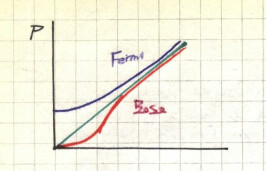
\includegraphics[scale=0.5]{images/1606329551.jpg}


El $C_V$ es continuo. Veamos que da
\[
	T<T_C \qquad \frac{C_V}{Nk} \propto T^{3/2}
\]
\[
	T=T_C \qquad \frac{C_V}{Nk} \approx 1.925 > \frac 3 2
\]
\[
	T>T_C \qquad \dpar{}{T}\left( \frac{3}{2} T \frac{g_{5/2}(z)}{g_{3/2}(z)} \right) \frac{C_V}{Nk} 
\]


% \bibliographystyle{CBFT-apa-good}	% (uses file "apa-good.bst")
% \bibliography{CBFT.Referencias} % La base de datos bibliográfica

\end{document}
